% Created 2021-09-12 Sun 22:48
% Intended LaTeX compiler: xelatex
\documentclass[letterpaper]{article}
\usepackage{graphicx}
\usepackage{grffile}
\usepackage{longtable}
\usepackage{wrapfig}
\usepackage{rotating}
\usepackage[normalem]{ulem}
\usepackage{amsmath}
\usepackage{textcomp}
\usepackage{amssymb}
\usepackage{capt-of}
\usepackage{hyperref}
\usepackage[margin=1in]{geometry}
\usepackage{fontspec}
\usepackage{indentfirst}
\setmainfont[ItalicFont = LiberationSans-Italic, BoldFont = LiberationSans-Bold, BoldItalicFont = LiberationSans-BoldItalic]{LiberationSans}
\newfontfamily\NHLight[ItalicFont = LiberationSansNarrow-Italic, BoldFont       = LiberationSansNarrow-Bold, BoldItalicFont = LiberationSansNarrow-BoldItalic]{LiberationSansNarrow}
\newcommand\textrmlf[1]{{\NHLight#1}}
\newcommand\textitlf[1]{{\NHLight\itshape#1}}
\let\textbflf\textrm
\newcommand\textulf[1]{{\NHLight\bfseries#1}}
\newcommand\textuitlf[1]{{\NHLight\bfseries\itshape#1}}
\usepackage{fancyhdr}
\pagestyle{fancy}
\usepackage{titlesec}
\usepackage{titling}
\makeatletter
\lhead{\textbf{\@title}}
\makeatother
\rhead{\textrmlf{Compiled} \today}
\lfoot{\theauthor\ \textbullet \ \textbf{2021-2022}}
\cfoot{}
\rfoot{\textrmlf{Page} \thepage}
\titleformat{\section} {\Large} {\textrmlf{\thesection} {|}} {0.3em} {\textbf}
\titleformat{\subsection} {\large} {\textrmlf{\thesubsection} {|}} {0.2em} {\textbf}
\titleformat{\subsubsection} {\large} {\textrmlf{\thesubsubsection} {|}} {0.1em} {\textbf}
\setlength{\parskip}{0.45em}
\renewcommand\maketitle{}
\author{Houjun Liu}
\date{\today}
\title{Lipids}
\hypersetup{
 pdfauthor={Houjun Liu},
 pdftitle={Lipids},
 pdfkeywords={},
 pdfsubject={},
 pdfcreator={Emacs 28.0.50 (Org mode 9.4.4)}, 
 pdflang={English}}
\begin{document}

\maketitle


\section{Lipids}
\label{sec:org47d6da1}
\subsection{Pentaine}
\label{sec:org5ce29f9}
\begin{figure}[htbp]
\centering
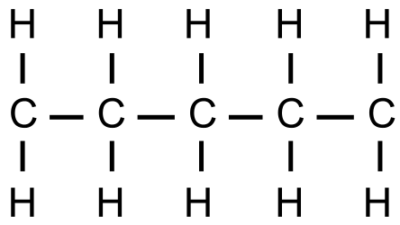
\includegraphics[width=.9\linewidth]{./pentane-plus-market-400x225.png}
\caption{pentane-plus-market-400x225.png}
\end{figure}

A non-polar molecule that build up the fundamentals of lipids.

\begin{itemize}
\item Non polar
\item Will only have LDF
\item Hydrophobic

\begin{itemize}
\item Because it is non polar, will only have LDF
\item So, water's dipole moment makes it not attractive to pentaine
\item Large surface area of pentaine will result in more LDF (bigger
surface area => more opportunities to LDF), so pentaines will more
likely to LDF with other pentains if given the choice between
pentain vs. water
\end{itemize}
\end{itemize}

\noindent\rule{\textwidth}{0.5pt}

\textbf{and now, a note on LDF}

Pentaine => Carbon-Carbon bonds has 0 EN difference w/ even distribution
of electrons

\begin{itemize}
\item Electrons are randomly within their 3D shape
\item So, when electrons are accidentally concentrated, a dipole moment will
temporarily form
\end{itemize}

\noindent\rule{\textwidth}{0.5pt}

\subsection{And now, actually lipids}
\label{sec:org35367fa}
Lipids are built up from peintaine molecules. You could also take many
of these lipids + other elements to build up more complicated,
hydrophobic/phillic structures.

\href{KBhBIO101StructuresOfLipids.org}{KBhBIO101StructuresOfLipids}
\end{document}
